\chapter[Synergy with WFIRST]{Synergy with WFIRST}
\def\chpname{wfirst}\label{chp:\chpname}

Chapter editor:
\credit{jasondrhodes}.

Contributing authors:
\credit{rubind},
\credit{davidpbennett},
\credit{mtpenny},
{\it Rachel Street}.

\section*{Summary}
\addcontentsline{toc}{section}{~~~~~~~~~Summary}

WFIRST will launch in $\sim$ 2025 for a 6 year mission to explore dark energy, find and characterize exoplanets, and take wide, deep infrared surveys of the galactic and extragalactic sky.  WFIRST was recognized by the Astro2010 Decadal Survey as an excellent NIR complement to LSST's optical capabilities.  Together, the two observatories can accomplish significantly more (and better) science than either can alone. Accomplishing this will require coordinated observations.  We have identified three areas of proposed coordination: 1. Early coverage of the $>2000$ square degree WFIRST High Latitude Survey to the full optical depth for enhanced photometric redshifts for both LSST and WFIRST; 2. Coordinated LSST optical observations in the WFIRST supernova discovery fields; 3. Precursor, simultaneous, and follow-up observations of the WFIRST microlensing fields near the galactic bulge.


% --------------------------------------------------------------------

\section{Introduction}
\label{sec:wfirst:intro}

% Introduce, with a very broad brush, this chapter's science projects,
% and why it makes sense for them to be considered together.

The Wide Field Infrared Survey Telescope (WFIRST) is a NASA mission that
entered Phase A in February 2016.  WFIRST was the highest recommendation
for large space missions in the 2010 New Worlds New Horizons Decadal
Survey.  That recommendation envisioned a wide-field observatory with
near infrared (NIR) capabilities to complement LSST's optical
capabilities; the Decadal Survey recognized the obvious synergy between
WFIRST and LSST.  WFIRST's design has evolved since 2010 and the design
being pursued for a mid-2020s launch uses an existing $2.4$m telescope
donated to NASA, giving WFIRST capabilities not envisioned by the
Decadal Survey.  WFIRST has 3 primary science objectives:

\begin{itemize}
\item Determine the nature of the dark energy that is driving the
current accelerating expansion of the universe using a combination of
weak lensing, galaxy clustering (including Baryon Acoustic Oscillations
and Redshift Space Distortions), and supernovae type Ia (SN).
\item Study exoplanets through a statistical microlensing survey and via
direct imaging and spectroscopy with a coronagraph.
\item Perform NIR surveys of the galactic and extragalactic sky via a
Guest Observer program.
\end{itemize}

WFIRST will be at L2 to enable the thermal stability needed for the
precise astrometric, photometric, and morphological measurements
required for these science goals. The baseline WFIRST mission
architecture is described in detail in the final report of the WFIRST
Science Definition Team (arxiv/1503.03757). The WFIRST Wide Field
Instrument(WFI) has a NIR focal plane with a $\sim0.28$ square degree
field of view made up 18 4k$\times$4k Teledyne H4RG NIR detectors and will
have imaging capabilities from $0.7-2$ microns and grism spectroscopy
capabilities from $1.35-1.89$ microns with $R\sim461\lambda$.  The WFI
also contains an Integral Field Channel (IFC) spectrometer with $R\sim100$
resoluton over the range $0.6-2$ microns for SN follow up. The exoplanet
coronagraph will have imaging ($0.43-0.97$ microns) and spectroscopic
($0.6-0.97 $ microns) capabilities with a contrast ratio of 1 part in a
billion.

WFIRST's  6 year primary mission is envisioned to have 2 years dedicated to a
$\sim2200$ square degree High Latitude Survey (HLS) for weak lensing and
galaxy clustering,  1 year of microlensing observations divided into 6
seasons, $0.6$ years of SN search and follow-up, one year dedicated to
the coronagraph and 1.4 years dedicated to competitively selected Guest
Observer observations. WFIRST has no expendables that would prevent an
extended mission of 10 years or longer, and an extended mission will likely be
given over entirely to Guest Observer observations.

The synergy with LSST is very promising indeed. In this chapter we aim
to  lay out three  specific projects in the three main WFIRST science
areas, and test the simulated LSST Observing
Strategies for their performance in each case. Then, we use these
results to design a suite of modified LSST Observing Strategies, which
we propose as new \OpSim simulation runs.



% --------------------------------------------------------------------

% ====================================================================
%+
% SECTION:
%    WFIRST_weaklensing.tex
%
% CHAPTER:
%    wfirst.tex
%
% ELEVATOR PITCH:
%    Explain in a few sentences what the relevant discovery or
%    measurement is going to be discussed, and what will be important
%    about it. This is for the browsing reader to get a quick feel
%    for what this section is about.
%
% COMMENTS:
%
%
% BUGS:
%
%
% AUTHORS:
%    Phil Marshall (@drphilmarshall)  - replace with your name and GitHub username!
%-  Jason Rhodes @jasondrhodes
% ====================================================================

\section{Cosmological Weak Lensing with WFIRST and LSST}
\def\secname{\chpname:weaklensing}\label{sec:\secname}

%note to Phil-  I am not sure if there will be another section that serves as an intro to WFIRST, but I am doing that here
%also, I think we should make this about more than just WL.  Can we change the name and focus of the section to the High Latitude Survey.  The driver %is still probably weak lensing!



\credit{jasondrhodes},
{\it and others to follow}

\textbf{Intro to WFIRST}

The Wide Field Infrared Survey Telescope (WFIRST) is a NASA mission that
entered Phase A in February 2016.  WFIRST was the highest recommendation
for large space missions in the 2010 New Worlds New Horizons Decadal
Survey.  That recommendation envisioned a wide-field observatory with
near infrared (NIR) capabilities to complement LSST's optical
capabilities; the Decadal Survey recognized the obvious synergy between
WFIRST and LSST.  WFIRST's design has evolved since 2010 and the design
being pursued for a mid-2020s launch uses an existing $2.4$m telescope
donated to NASA, giving WFIRST capabilities not envisioned by the
Decadal Survey.  WFIRST has 3 primary science objectives:

\begin{itemize}
\item Determine the nature of the dark energy that is driving the
current accelerating expansion of the universe using a combination of
weak lensing, galaxy clustering (including Baryon Acoustic Oscillations
and Redshift Space Distortions), and supernovae type Ia (SN).
\item Study exoplanets through a statistical microlensing survey and via
direct imaging and spectroscopy with a coronagraph.
\item Perform NIR surveys of the galactic and extragalactic sky via a
Guest Observer program.
\end{itemize}

WFIRST will be at L2 to enable the thermal stability required for the
precise astrometric, photometric, and morphological measurements
required for these science goals. The baseline WFIRST mission
architecture is described in detail in the final report of the WFIRST
Science Definition Team (arxiv/1503.03757). The Wide Field
Instrument(WFI) has a NIR focal plane with a $\sim0.28$ square degree
field of view made up 18 4k$\times$4k Teledyne H4RG NIR detectors will
have imaging capabilities from $0.7-2$ microns and grism spectroscopy
capabilities from $1.35-1.89$ microns with $R\sim461\lambda$.  The WFI
also contains an Integral Field Unit (IFU) spectrometer with $R\sim100$
resoluton over the range $0.6-2$ microns for SN follow up. The exoplanet
coronagraph will have imaging ($0.43-0.97$ microns) and spectroscopic
($0.6-0.97 $ microns) capabilities with a contrast ratio of 1 part in a
billion.

WFIRST's  6 year primary mission will have 2 years dedicated to a
$\sim2200$ square degree High Latitude Survey (HLS) for weak lensing and
galaxy clustering,  1 year of microlensing observations divided into 6
seasons, $0.6$ years of SN search and follow-up, one year dedicated to
the coronagraph and 1.4 years dedicated to competitively selected Guest
Observer observations. WFIRST has no expendables that would prevent an
extended mission of 10 years or longer, and an extended mission would be
given over entirely to Guest Observer observations.

\textbf{WFIRST's High Latitude Survey (HLS)}

WFIRST's HLS will cover 2200 square degrees in 4 NIR photometric filters
(3 of which will be sufficiently sampled for weak lensing shape
measurements) and NIR grism spectroscopy.  The benefits of overlapping
spectroscopic and photometric surveys for dark energy constraints and
systematics mitigation are strong.  The primary scientific driver of the
photometric portion of the WFIRST HLS is weakg gravitational lensing,
but there is a wide range of ancillary science that will be possible
with the publicly available WFIRST HLS data (see for instance, the SDT
report mentioned above).  However, the requirements on the HLS are
largely set by constraints from weak lensing measurements.  Each galaxy
in the WFIRST weak lesing survey needs to have an accurate photometric
redshift.  This requires optical photometry that reaches the depth of
the NIR photometry WFIRST will acquire ($J~27AB$).  \emph{Thus, the
WFIRST weak lensing survey will require the full  10-year LSST depth in
4 optical bands for optimal photometric redsfhift determination}.

There is strong benefit not jsut to WFIRT, but to LSST, in coordinating
observations of the WFIRST HLS survey field. The combination of
full-depth LSST data and WFIRST HLS NIR data will provide the gold
standard in photo-zs.  Furthermore, WFIRST grism observations over the
same area will provide many millions of high quality slitless spectra
and WFIRST’s IFU can be run in parallel with WFI observations to provide
many more very accurate spectroscopic redshifts in the survey area.
Thus, the WFIRST photometric data will help to provide better LSST
photo-zs and  WFIRST will also provide many of the spectra needed for a
training set to calibrate the photo-zs for both missions.  A further
benefit to LSST might be the reduced need for LSST observations at the
reddest end of the LSST wavelength range (the z and y filters), where
both the atmosphere and the physics of CCDs make ground-based
observations less efficient than what WFIRST can achieve. Finally, the
joint processing of LSST and WFIRST data will provide better object
deblending parameters than LSST can achieve alone; WFIRST will be able
to provide a morphological prior for the deblending of LSST images.

% --------------------------------------------------------------------

\subsection{Target measurements and discoveries}
\label{sec:\secname:targets}

We propose an acceleration of the LSST survey over about $10\%$ of the
LSST survey area (the $\sim2200$ WFIRST HLS) such that the full LSST ten
years survey depth is reached on a timescale that maximizes the joint
usefulness of LSST and WFIRST data on that area.  Assuming the two year
WFIRST HLS is taken in the first four years of a WFIRST mission that
launches in 2024, this would require reaching full LSST depth over that
area in $\sim2028$ rather than $\sim2032$. Since the HLS area is roughly
$1/8$ as large as the LSST ``Main Survey"'' region, this could be
achieved by devoting 1.25 years of LSST observations to the HLS area,
assuming that it covers a wide enough range of Right Ascension.  More
practically, it could be achieved by devoting 25\% of LSST observing
time to this area during each of the first 5 years of the LSST survey,
which doubles the time it would naturally be observed during those years
at a modest reduction in coverage of the rest of the Main Survey area
during that time period.   Given existing plans to speed up the LSST
cadence over small sub-areas of the LSST survey, this may only require
coordination of the locations of the accelerated LSST area and the
WFIRST HLS. As LSST and WFIRST progress, there is a mutual benefit in
continuing discussions about the optimal joint observation schedule.

It is possible that the WFIRST data might allow for shallower LSST data
in the reddest LSST filter in the overlap region, and this must be
quantified.


% --------------------------------------------------------------------

\subsection{Metrics}
\label{sec:\secname:metrics}

A simple, first order metric would be the amount of LSST/WFIRST
overlapping survey area that reaches the full LSST depth when the WFIRST
HLS is completed.  Such a metric is straightforward, but not
quantitative until the 2020s, when the WFIRST launch date and survey
plan is more definite.  A slightly more complicated metric could include
the pace at which the overlapping LSST/WFIRST survey areas are both
taken to full depth, since this would make each data set maximally
useful to the US community (or anyone with immediate access to both
WFIRST and LSST data).  WFIRST data is unlikely to have any proprietary
period.  Current plans call for the WFIRST HLS to be conducted in
multple passes, but the exact survey pattern is still undecided, so this
metric is also not quantifiable yet.

There may be some reduced need for the the LSST reddest bands in the
WFIRST HLS overlap area, which should also be folded into the metric.

% --------------------------------------------------------------------

\subsection{OpSim Analysis}
\label{sec:\secname:analysis}

The default survey strategy would only achieve the full LSST photometric
depth over the WFIRST HLS after 10 years of survey ($\sim2032$).


% --------------------------------------------------------------------

\subsection{Discussion}
\label{sec:\secname:discussion}

Increasing the cadence of the LSST survey over $\sim10\%$ of the LSST
survey has science benefits that go far beyond the LSST/WFIRST synergy
described here.  There are benefits to certain aspects of time-domain
science.  Every effort should be made to coordinate all discussions of
increased survey cadence (resulting in full LSST depth well before 10
years) over sub-areas of the LSST survey footprint.  Specific attention
should be paid to whether the accelerated portions of the LSSt survey
can completely overlap the WFIRST HLS, and whether the position of the
WFIRST HLS can be determined, in part, by other science drivers within
LSST.  This will require close LSST and WFIRST coordination at the
Project levels.


% ====================================================================

\navigationbar


% PJM: commented out pending check-in from Dave Rubin
% ====================================================================
%+
% SECTION:
%    WFIRST_supernovae.tex
%
% CHAPTER:
%    wfirst.tex
%
% ELEVATOR PITCH:
%-
% ====================================================================

\section{Supernova Cosmology with WFIRST and LSST}
\def\secname{\chpname:supernovae}\label{sec:\secname}

\credit{rubind}

% This individual section will need to describe the particular
% discoveries and measurements that are being targeted in this section's
% science case. It will be helpful to think of a ``science case" as a
% ``science project" that the authors {\it actually plan to do}. Then,
% the sections can follow the tried and tested format of an observing
% proposal: a brief description of the investigation, with references,
% followed by a technical feasibility piece. This latter part will need
% to be quantified using the MAF framework, via a set of metrics that
% need to be computed for any given observing strategy to quantify its
% impact on the described science case. Ideally, these metrics would be
% combined in a well-motivated figure of merit. The section can conclude
% with a discussion of any risks that have been identified, and how
% these could be mitigated.
%
% A short preamble goes here. What's the context for this science
% project? Where does it fit in the big picture?

The WFIRST SN survey seeks to measure thousands of SNe Ia with excellent systematics control over a two-year period. The SDT outlined a three-tiered cadenced imaging survey: wide to $z=0.4$ (27.44 square degrees), medium to $z=0.8$ (8.96 square degrees), deep to $z=1.7$ (5.04 square degrees). SNe discovered in the imaging would followed with IFU spectrophotometry, helping to monitor changes in SN physical parameters and the extinction distribution with redshift. However, due to the slew time (now believed to be higher than was used in the SDT survey), and high read noise in short exposures, the wide survey was very inefficient, spending a bit more than half of its time on slews, while the medium survey would spend a significant fraction of its time slewing. However, the LSST DDFs offer a path to high signal-to-noise, well calibrated, multi-band optical imaging over an even larger area than WFIRST can survey. If the wide and medium tiers are replaced with LSST DDF discoveries, then WFIRST can offer spectrophotometry (with good host-galaxy subtraction) for $\sim$ 2,000 LSST SNe, with screening spectra for $\sim$ 1-2,000 more. As the WFI and IFU operate in parallel, this survey could provide sparsely sampled NIR imaging for $\sim$ 5,000 SNe up to $z = 1$ at the same time as the spectroscopy. The joint survey would thus provide systematics control (almost certainly better than either survey alone), as well as a cross-check of LSST photometric typing and host-galaxy-only redshift assignment.

% --------------------------------------------------------------------

\subsection{Target measurements and discoveries}
\label{sec:\secname:targets}

% Describe the discoveries and measurements you want to make.
%
% Now, describe their response to the observing strategy. Qualitatively,
% how will the science project be affected by the observing schedule and
% conditions? In broad terms, how would we expect the observing strategy
% to be optimized for this science?



All these goals can be met with $\sim 3$ day rest-frame cadence ($\sim 5$ observer-frame days). LSST would measure NUV to rest-frame $V$-band (with WFIRST providing redder wavelength coverage), or observer-frame $grizY$. For a plausible SN Ia (based on the rising light curve), a series of typing/sub-typing spectra would be triggered, with increasing depth, as the confidence grew that the transient was a SN Ia. DR: in my simulations, I've assumed a depth for each filter of 26th magnitude (probably not realistic for $Y$-band, but very feasible for the other filters); is this too shallow? LSST would contribute 4 transients per day to the pool of objects observed by WFIRST. In practice, the LSST DDFs will contain more SNe Ia than this, so a random sample (perhaps sculpted in redshift) should be sent for observations.

% --------------------------------------------------------------------

\subsection{Metrics}
\label{sec:\secname:metrics}

% Quantifying the response via MAF metrics: definition of the metrics,
% and any derived overall figure of merit.

The primary metrics are based on constraining cosmological parameters; the DETF FoM is standard (although other cosmological FoMs can be constructed using eigenmode constraints). For the joint observations proposed here, we anticipate an increase in the FoM of about 20\% (DR is still working to optimize the WFIRST side of the joint survey for the best possible constraints). The cosmological metric will be composed of several (related) metrics: the fraction of non SNe Ia mistakenly sent to WFIRST for followup, the number of SNe Ia sent to WFIRST, but lost due to weather gaps, and the fraction of SNe sent to WFIRST, but lacking the light-curve sampling to constrain key light-curve parameters (date of maximum, rise time and decline time, etc.).

% --------------------------------------------------------------------

%\subsection{OpSim Analysis}
%\label{sec:\secname:analysis}

% OpSim analysis: how good would the default observing strategy be, at
% the time of writing for this science project?


% --------------------------------------------------------------------

%\subsection{Discussion}
%\label{sec:\secname:discussion}

% Discussion: what risks have been identified? What suggestions could be
% made to improve this science project's figure of merit, and mitigate
% the identified risks?


% ====================================================================

\navigationbar


% ====================================================================
%+
% SECTION:
%    WFIRST_microlensing.tex
%
% CHAPTER:
%    wfirst.tex
%
% ELEVATOR PITCH:
%
%
% AUTHORS:
%    David Bennett(@davidpbennett)
%-
% ====================================================================

\section{Exoplanetary Microlensing with WFIRST and LSST}
\def\secname{\chpname:microlensing}\label{sec:\secname}

\credit{davidpbennett},
\credit{mtpenny},
{\it Rachel Street}.

Perhaps the most exciting discovery to come out of gravitational
microlensing surveys is the discovery of a large population of ``rogue"
planets by the MOA Collaboration (Sumi et al.\ 2011). These planets
are isolated in the sense that no host star can be detected
by microlensing. Depending on the peak magnification and light curve
coverage, this can imply that a host must be $> 10\,$AU or $> 100\,$AU,
and Bennett et al.\ (2012) have argued that the median separation
of possible host stars is likely to be $> 30\,$AU.
Further observations by both the MOA and OGLE collaborations provide
a qualitative confirmation of this result, as dozens of additional
short timescale events have been discovered by the MOA and OGLE
alert systems, but we await details of the implied rogue planet
populations that will come from detailed analyses of bot the MOA
and OGLE samples.

A major weakness with the microlensing data that indicates this
large population of rogue planets is that, thus far, the properties
of this population have only been inferred by their Einstein radius
crossing time, $t_E$, distribution. But, the Einstein radius crossing
time depends not only on the lens mass, but also on its distance and
transverse velocity. As a result, we cannot directly infer the mass or distance
distribution of the rogue planet sample.

Our understanding of the rogue planet distribution can be greatly improved
by measuring the microlensing parallax effect (Gould et al.\ 1992;
Alcock et al.\ 1995). The microlensing parallax effect can be described
by the transverse relative lens-source velocity, ${\bf v}_{\rm \perp}$, projected
to the position of the observer,
\begin{equation}
\tilde{\bf v} = {\bf v}_{\rm \perp} D_S/(D_S-D_L) \ , \label{eq-vp}
\end{equation}
where $D_L$ and $D_S$ are the lens and source distances, respectively.
Typically, microlensing parallax
is measured using the orbital motion of the Earth, but it can also be
measured using light curve observations from telesopes at different locations
in the Solar System (Dong et al.\ 2007; Calchi Novati et al.\ 2015) or
even different locations on Earth (Gould et al.\ 2009). However, in the
case of microlensing by planetary mass objects, the event durations are
too short to allow a significant light curve change due to the Earth's
orbital motion, but the near simultaneous observations from Earth and a
satellite orbiting at the Earth-Sun L2 point (where WFIRST will orbit) does
allow the measurement of microlensing parallax signals due to planetary mass
lenses (Gould, Gaudi \& Han, 2003).

When a microlensing parallax signal is measured, the $\tilde{\bf v}$ value
can generally distinguish between bulge and disk lenses, as $\tilde{\bf v}$
generally points in the direction of the Galactic disk rotation and has
a magnitude of $\tilde{v} \ltsim 200\,$km/sec for a lens in the
disk, while for a lens in the bulge, the magnitude of the projected velocity
is $\tilde{v} \gtsim 200\,$km/sec. A microlensing parallax measurement also
yields a mass distance relationship,
\begin{equation}
   M_L = {\tilde{v}^2 t_E^2 c^2 \over 4 G} {D_S-D_L \over D_L D_S} \ .
   \label{eq-m_vt}
\end{equation}
Because the $\tilde{\bf v}$ value places a fairly strong constraint
on $D_L$ and the source is very likely to be in the bulge, equation~\ref{eq-m_vt}
generally provides a good constraint on the lens mass. But, for some
events, we can do even better. For high magnification events or events
with low-mass lenses, the finite angular size of the source star is
resolved, and the light curve provides a measurement of the source
radius crossing time, $t_*$. This allows the angular Einstein radius
to be determined, $\theta_E = t_E \theta_*/t_*$, where the angular
source radius, $\theta_*$ can be determined from the color and brightness
of the source star (Boyajian et al.\ 2014). When both $\tilde{v}$ and
$\theta_E$, the mass of the lens is measured to be
\begin{equation}
M_L = {c^2\over 4G} \tilde{v} t_E \theta_E = {\theta_E\tilde{v} t_E \over (8.1439\,{\rm mas\, AU})} M_{\odot} \ .
\label{eq-m}
\end{equation}
Figure~\ref{fig-lc} shows an example of the light curves for one of the
rougue planets with a mass determined by simultaneous WFIRST and LSST
observations.

\begin{figure}[t]
\centering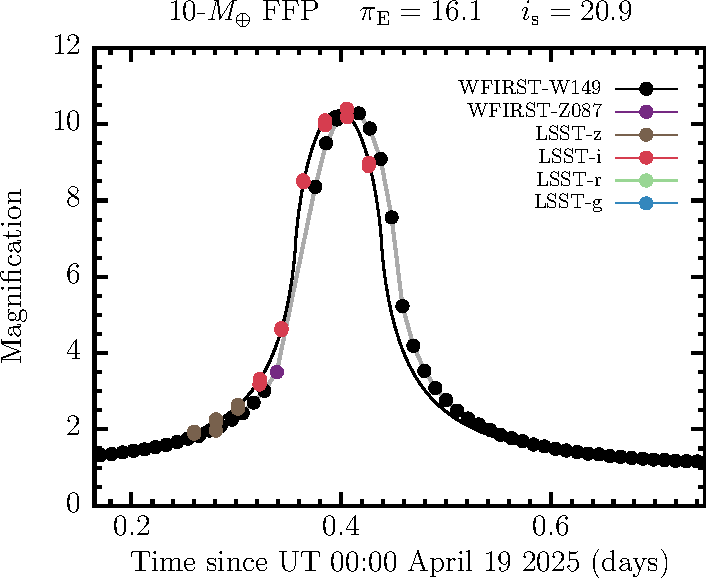
\includegraphics[width=0.5\linewidth]{figs/WFIRST/lsst_lsstm+10_0_7220351_320_det_lc.pdf}
\caption{The light curve of a $10 M_{\oplus}$ planet with a microlensing parallax
mass measurement from simultaneous WFIRST and LSST observations.
\label{fig-lc}}
\end{figure}

We propose simultaneous high cadence observations of the WFIRST microlensing fields
(which should be covered by a single LSST pointing) by LSST during each
of the six 72-day WFIRST exoplanet microlensing survey sessions. These
will allow microlensing parallax measurements to determine the distances
and masses of a representative sub-sample of the rogue planets found by
the WFIRST microlensing survey. These measurements will be crucial for
the interpretation of WFIRST's rogue planet discoveries, and they
cannot be obtained by another method.

We also propose continuous monitoring of the WFIRST microlensing fields
at a cadence of one observation per day
starting a year before and ending a year after the WFIRST microlensing.
This will allow us to search for microlensing signals of possible
host stars for the detected rogue planet candidates. Such signals will
appear as seperate microlensing signals long before or after the apparent
rogue planetary signals. They cannot be detected by WFIRST due to the
limited 72 day WFIRST observing windows.

% This individual section will need to describe the particular
% discoveries and measurements that are being targeted in this section's
% science case. It will be helpful to think of a ``science case" as a
% ``science project" that the authors {\it actually plan to do}. Then,
% the sections can follow the tried and tested format of an observing
% proposal: a brief description of the investigation, with references,
% followed by a technical feasibility piece. This latter part will need
% to be quantified using the MAF framework, via a set of metrics that
% need to be computed for any given observing strategy to quantify its
% impact on the described science case. Ideally, these metrics would be
% combined in a well-motivated figure of merit. The section can conclude
% with a discussion of any risks that have been identified, and how
% these could be mitigated.

% A short preamble goes here. What's the context for this science
% project? Where does it fit in the big picture?


% --------------------------------------------------------------------

\subsection{Target measurements and discoveries}
\label{sec:\secname:targets}

We will point at a single field, centered on the WFIRST microlensing
fields, and this should cover all 10 WFIRST microlensing fields.

For our preliminary estimates of the high cadence observing, we assume
that the bulge is observed every 30 minutes when the bulge is at
an airmass of $< 2.5$ for 76-day observing runs (each 72-day WFIRST observing
season plus 2 days on either side). Each visit consists of 3 exposures,
one 2 sec exposure followed by two 15 sec exposures. With a 2 sec readout
and 1 sec for the shutter to open and close, this comes to 42 sec on target
per visit (since the final readout can be done while slewing).
If we assume a 30 deg slew in Azimuth before and after each ML pointing, the slews
to and from the target should take 22 sec, which is 12 sec above the average. So,
each observation will take 66 sec out of the regular observing sequence.
The number of observations per night, assuming a 30 minute cadence, for
a Spring, 2025 observing session are given in \autoref{tab:wfirst_ml_survey}. We will require
that these observations be taken in the $riz$ or $y$ filters with at
least 3 (or 0) observations in each filter per night. The total number
of observations with this observing plan is 649 or 11.9 hour per
72-day observing session or 3894 observations and 71.4 hours for
all the high cadence observations that we propose.

\begin{table}
\begin{tabular}{ c c }
{\bf days} & {\bf Observations} \\
\hline
Feb 10-16     &  3 \\
Feb 17-23     &  4 \\
Feb 24-Mar 1  &  5 \\
Mar 2-8       &  6 \\
Mar 9-14      &  7 \\
Mar 15-21     &  8 \\
Mar 22-28     &  9 \\
Mar 29-Apr 4  & 10 \\
Apr 5-10      & 11 \\
Apr 11-17     & 12 \\
Apr 18-24     & 13 \\
Apr 25-28     & 14 \\
\end{tabular}
\caption{Observations per night at 30 minute cadence for a Spring
WFIRST microlensing survey.}
\label{tab:wfirst_ml_survey}
\end{table}

The low-cadence (1 observation per day) observations taken when WFIRST
is not observing, would consist of 1270 observations if we assume that
the observations are not taken during the time when the $u$ filter is
on the telescope (this is assumed to be 1/6 of the time). The low-cadence
off-season observations then total 23.3 hours, for a grand total of
95.7 hours over 8 years.

These observing plans can be altered by changing the cadence of the high
cadence observations from once every 30 minutes to once every 15, 60,
or 120 minutes, or we could change the number of WFIRST microlensing
observing seasons that were covered. We have not yet simulated the
different observing cadences, however.

% --------------------------------------------------------------------

\subsection{Metrics}
\label{sec:\secname:metrics}

\autoref{tab:wfirst_ml_results}
shows the results of our simulations of the combined WFIRST-LSST
observing program. We assume that there is 1 planet per main sequence
star at each of $1\,M_\oplus$, $10\,M_\oplus$, and $100\,M_\oplus$.
This is the 1-$\sigma$ lower limit found by Sumi et al.\ (2011) at
$M_L \approx 300\,M_\oplus$, and the rogue planet mass function is
thought to increase toward lower masses, so this is a conservative
assumption. The first row gives the number of events that will be
observed by WFIRST. The second row gives the number of these events
with SDSS-$i \leq 23$, which were the only events included in the
LSST simulations. The third and fourth rows give the number of these events
with LSST-WFIRST microlensing parallax measurements and the number
with full mass measurements. It is these rows that indicate the
value of the LSST observations.

\begin{table}
\begin{tabular}{lcccc}
Category & $100\,M_\oplus$ & $10\,M_\oplus$ & $1\,M_\oplus$ & Total \\
\hline
WFIRST-events    &   417   &         127    &         33    &  577  \\
$i \leq 23$      &    88   &          30    &         13    &  131  \\
$\pi_E$ measured &    22   &           8.2  &          2.7  &   32.9 \\
$M_L$ measured   &    5.9  &           3.4  &          1.5  &   10.8 \\
\end{tabular}
\caption{Number of rogue planets of the given mass detected, assuming
one such planet per main sequence star.}
\label{tab:wfirst_ml_results}
\end{table}

We can see from the final column that the LSST observations should
yield more than 30 rogue planet microlensing parallax measurements and
more than 10 rogue planet mass measurements. And these are measurements
that cannot be made by other methods. In addition, this program would
also yield masses for a somewhat larger number of bound planets
(Gould, Gaudi \& Han 2003), although many of these will have their
masses determined by other means as well.

For a figure of merit, we select the product of the number of $\pi_E$
and $M_L$, which is 355 for our straw man program.

% Quantifying the response via MAF metrics: definition of the metrics,
% and any derived overall figure of merit.

% % --------------------------------------------------------------------
%
% \subsection{OpSim Analysis}
% \label{sec:\secname:analysis}
%
% OpSim analysis: how good would the default observing strategy be, at
% the time of writing for this science project?
%
%
% % --------------------------------------------------------------------
%
% \subsection{Discussion}
% \label{sec:\secname:discussion}
%
% Discussion: what risks have been identified? What suggestions could be
% made to improve this science project's figure of merit, and mitigate
% the identified risks?
%
%
% ====================================================================

\navigationbar


% --------------------------------------------------------------------

% ====================================================================
%+
% SECTION:
%    WFIRST_proposals.tex
%
% CHAPTER:
%    wfirst.tex
%
% ELEVATOR PITCH:
%    Maximizing the overlap between LSST and WFIRST is likely to be a fruitful
%    approach to modifying the LSST observing strategy. Let's pull together the
%    findings from the three WFIRST science cases and propose some OpSim
%    experiments.
%
%-
% ====================================================================
% 
% \section{Maximizing the Synergy between WFIRST and LSST}
% \def\secname{\chpname:proposals}\label{sec:\secname}
%
% \credit{jasondrhodes}
%
% In the previous sections, we introduced figures of merit for each WFIRST
% science project, and tested the existing LSST observing strategies for
% their performance. In the process we learned some of the shortcomings of the
% baseline LSST strategy, and suggested some alternative cadence
% options. In this section, we will pull those suggestions together to propose a
% suite of new \OpSim experiments.
%
% % Make table here.
%
% % ====================================================================
%
% \navigationbar


% --------------------------------------------------------------------

\navigationbar
